

\begin{center}
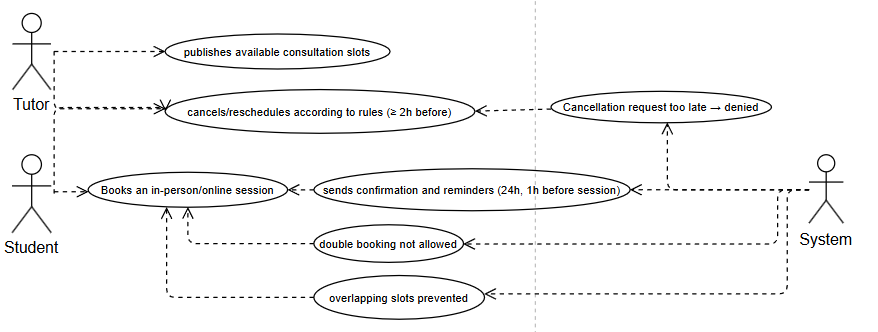
\includegraphics[width=0.9\linewidth]{images/UC-03.png}
\end{center}

\begin{center}
\textbf{Figure 4:}  Session Scheduling Management
\end{center}

\begin{table}[H]
\centering
\renewcommand{\arraystretch}{1.3}
\begin{tabular}{|p{3cm}|p{11cm}|}
\hline
\textbf{Use-case ID} & UC-03a \\
\hline
\textbf{Use-case name} & Publish and Manage Tutor Availability \\
\hline
\textbf{Overview} & To allow a tutor to create, edit, and manage available consultation slots, while the system prevents overlapping sessions and validates scheduling rules. \\
\hline
\textbf{Actors} & Tutor, System \\
\hline
\textbf{Preconditions} &
\begin{itemize}
    \item Tutor is authenticated in the system.
    \item The scheduling database is accessible.
\end{itemize} \\
\hline
\textbf{Trigger} & Tutor selects “Set Availability” or modifies existing slots. \\
\hline
\textbf{Main Flow (Steps)} &
\begin{enumerate}
    \item Tutor publishes available consultation slots.
    \item System checks for overlapping slots.
    \item If no conflicts are found, slots are confirmed and saved.
    \item Tutor may later edit or delete slots before they are booked.
\end{enumerate} \\
\hline
\textbf{Postconditions} &
\begin{itemize}
    \item Valid time slots are stored in the system and visible to students.
\end{itemize} \\
\hline
\textbf{Alternative Flows} &
\begin{itemize}
    \item[AF1:] Overlapping slot detected → system rejects slot creation and displays conflict message.
\end{itemize} \\
\hline
\textbf{Exception Flows} &
\begin{itemize}
    \item Database or connection error → slot creation aborted, system logs error.
\end{itemize} \\
\hline
\end{tabular}
\caption{Use Case UC-03a: Publish and Manage Tutor Availability}
\end{table}


\begin{table}[H]
\centering
\renewcommand{\arraystretch}{1.3}
\begin{tabular}{|p{3cm}|p{11cm}|}
\hline
\textbf{Use-case ID} & UC-03b \\
\hline
\textbf{Use-case name} & Session Booking, Reminders, and Cancellation Rules \\
\hline
\textbf{Overview} & To allow a student to book an in-person or online session with a tutor, receive automatic confirmations and reminders, and manage cancellations or reschedules according to defined rules. \\
\hline
\textbf{Actors} & Student, Tutor, System \\
\hline
\textbf{Preconditions} &
\begin{itemize}
    \item Tutor has published available slots.
    \item Student is authenticated and matched with a tutor.
\end{itemize} \\
\hline
\textbf{Trigger} & Student initiates a booking or a cancellation/reschedule request. \\
\hline
\textbf{Main Flow (Steps)} &
\begin{enumerate}
    \item Student views tutor’s available consultation slots.
    \item Student selects a preferred slot and submits booking.
    \item System checks for double booking or slot conflicts.
    \item Booking is confirmed, and notifications are sent to student and tutor.
    \item System automatically sends reminders (24h and 1h before the session).
    \item If cancellation or reschedule is requested \(\geq 2h\) before session it is approved.
\end{enumerate} \\
\hline
\textbf{Postconditions} &
\begin{itemize}
    \item Session status updated (booked, rescheduled, or cancelled).
    \item All notifications are logged and delivered.
\end{itemize} \\
\hline
\textbf{Alternative Flows} &
\begin{itemize}
    \item[AF1:] Cancellation request too late (<2h before) → denied with reason.
    \item[AF2:] Tutor unavailable → student notified and slot reopened.
\end{itemize} \\
\hline
\textbf{Exception Flows} &
\begin{itemize}
    \item Network or database failure → transaction aborted, retry suggested.
\end{itemize} \\
\hline
\end{tabular}
\caption{Use Case UC-03b: Session Booking, Reminders, and Cancellation Rules}
\end{table}
